%%%%%%%%%%%%%%%%%%%%%%%%%%%%%%%%%%%%%%%%%%%%%%%%%%%%%%%%%%%%%%%%%%%%%%%%%
%  Content: Main file of thesis template (master/enginering).
%  Author: Tomasz Kubik <tomasz.kubik@pwr.edu.pl>
%  Date: 9 Feb 2021
%  Version: 0.5
%%%%%%%%%%%%%%%%%%%%%%%%%%%%%%%%%%%%%%%%%%%%%%%%%%%%%%%%%%%%%%%%%%%%%%%%%

\documentclass[a4paper,onecolumn,oneside,12pt,extrafontsizes]{memoir}
% In oder to prepare the manuscript for archives (2x1, double printed) you can:
% a) produce normal pdf, then convert it to pdf with two pages on one phisical page (solution suggested)
%
%   This can be done by:
%   - printing from Adobe Acrobat Reader with option "Multiple"
%   - using psutils
%
%      Windows (assuming that you have MiKTeX installed with the package pakiet miktex-psutils-bin-x64-2.9):
%        "c:\Program Files\MiKTeX 2.9\miktex\bin\x64\pdf2ps.exe" Dyplom.pdf Dyplom.ps
%        "c:\Program Files\MiKTeX 2.9\miktex\bin\x64\psnup.exe" -2 Dyplom.ps Dyplom2.ps
%        "c:\Program Files\MiKTeX 2.9\miktex\bin\x64\ps2pdf.exe" Dyplom2.ps Dyplom2.pdf
%        Del Dyplom2.ps Dyplom.ps
%
%     Linux:
%        pdf2ps Dyplom.pdf - | psnup -2 | ps2pdf - Dyplom2.pdf
%
%
% b) produce 'reduced' pdf by settning smaller fonts in the document class definition (it changes the formating thus it is not suggested)
%
%   Use of the following commands instead of original one:
%   \documentclass[a4paper,onecolumn,twoside,10pt]{memoir} 
%   \renewcommand{\normalsize}{\fontsize{8pt}{10pt}\selectfont}

\usepackage[cp1250]{inputenc} % Use it if you work with cp1250 file encoding
%\usepackage[utf8]{inputenc} % Switch to if if you work with UTF8 file encoding
\usepackage[T1]{fontenc}
\usepackage[polish,english]{babel} % The order of attributes matters (for thesis in english then attribute 'english' must be at the end)
%\DisemulatePackage{setspace}
\usepackage{setspace}
\usepackage{tabularx}
\usepackage{color,calc}
%\usepackage{soul} % packege with commands for text highliting (rather not required)

\usepackage{ebgaramond} % package with garamond font (required on the title page)

%% Accorging to the rules the main font of the thesis should be Times.
%% In order to achieve it we use tgtermes font that offers shapes: normal, bold, italic, italic bold.
%% There is no slanted shape.
%% If you use slanted font in the text (typing \textsl{} command), then LaTeX will substitute it with a standard font giving you a warning.
%% Additionally tgtermes works for the running text. All maths (formulas, equations) will be rendered with a default font for math.
%% If you with to change the font for math, you must to do it yourself.

%% After installation of tgtermes package there might be a need to update font and mapping information 
%% This can be don by running the following commands (as administrator)
%% initexmf --admin --update-fndb
%% initexmf --admin --mkmaps

\usepackage{pgfplots}
\pgfplotsset{width=15cm, compat=1.9}
\usepgfplotslibrary{external}
\tikzexternalize 
\usepackage{rotating}

\usepackage{tgtermes}   
\renewcommand*\ttdefault{txtt}

\usepackage{multicol} % Package for typing in multicolums
%%%%%%%%%%%%%%%%%%%%%%%%%%%%%%%%%%%%%%%%%%%%%%%%%%%
%% Packages for editing tables
%%%%%%%%%%%%%%%%%%%%%%%%%%%%%%%%%%%%%%%%%%%%%%%%%%%
\usepackage{tabularx}
% Use tabularx package only. Other packages left untouched !!!
% Thesis for sure can be edited without using them.
%\usepackage{longtable}
%\usepackage{ltxtable}
%\usepackage{tabulary}

%%%%%%%%%%%%%%%%%%%%%%%%%%%%%%%%%%%%%%%%%%%%%%%%%%%
%% Package for inserting source code fragments
%%%%%%%%%%%%%%%%%%%%%%%%%%%%%%%%%%%%%%%%%%%%%%%%%%%
\usepackage{listings} %
\usepackage{xpatch}
\makeatletter
\xpatchcmd\l@lstlisting{1.5em}{0em}{}{}
\makeatother
% Package delivers lstlisting environment which is highly configurable.
% Listings can be configured individually or globally, with the use of \lstset{} command 
% Is is strongly suggested to renred source code using typewriter font family \ttfamily
% More over, due to the longiness of sources, even after removing unnecessary parts, the font should be lowered. 
% Thus use \small (for short fragments) and \footnotesize (for longer framents)

\lstset{
  basicstyle=\small\ttfamily, % or basicstyle=\footnotesize\ttfamily
  %%columns=fullflexible,
	%%showstringspaces=false,
	%%showspaces=false,
  breaklines=true,
  postbreak=\mbox{\textcolor{red}{$\hookrightarrow$}\space}, 
  %%numbers=left,  % this and following lines are related to numbering and its rendering
  %%firstnumber=1, 
  %%numberfirstline=true, 
	%%xleftmargin=17pt,
  %%framexleftmargin=17pt,
  %%framexrightmargin=5pt,
  %%framexbottommargin=4pt,
	belowskip=.5\baselineskip
}

% If the edited file is not in cp1250 encoding, then there is a problem with Polish characters in the inserted code.
% Therefore, when working with files in UTF-8 encoding, you need to declare the mapping as follows (just unmark to use).
% Unfortunately, when this mapping is applied, there may be problems with syntax highlighting (see further comments). 
%%\lstset{literate=%-
%%{�}{{\k{a}}}1 {�}{{\'c}}1 {�}{{\k{e}}}1 {�}{{\l{}}}1 {�}{{\'n}}1 {�}{{\'o}}1 {�}{{\'s}}1 {�}{{\.z}}1 {�}{{\'z}}1 {�}{{\k{A}}}1 {�}{{\'C}}1 {�}{{\k{E}}}1 {�}{{\L{}}}1 {�}{{\'N}}1 {�}{{\'O}}1 {�}{{\'S}}1 {�}{{\.Z}}1 {�}{{\'Z}}1 
    %%{�}{{\"O}}1
    %%{�}{{\"A}}1
    %%{�}{{\"U}}1
    %%{�}{{\ss}}1
    %%{�}{{\"u}}1
    %%{�}{{\"a}}1
    %%{�}{{\"o}}1
    %%{~}{{\textasciitilde}}1
		%%{�}{{{\textemdash} }}1
%%}%{\ \ }{{\ }}1}


%% lstlisting allows you to style the syntax highlighting of selected languages.
%% This works by defining keywords and rules on how to display them.
%% Because it is a simple mechanism, it is sometimes difficult to achieve the quality as in IDE tools.
%% However, in most cases the results are satisfactory.
%% \ lstloadlanguages {% Check Documentation for further languages ... 
%%C,
%%C++,
%%csh,
%%Java
%%}

%% lstlisting supports some of the most popular languages by default.
%% Other languages must be added. Examples of definitions of languages and styles are given below. 


\definecolor{lightgray}{rgb}{.9,.9,.9}
\definecolor{darkgray}{rgb}{.4,.4,.4}
\definecolor{purple}{rgb}{0.65, 0.12, 0.82}
\definecolor{javared}{rgb}{0.6,0,0} % for strings
\definecolor{javagreen}{rgb}{0.25,0.5,0.35} % comments
\definecolor{javapurple}{rgb}{0.5,0,0.35} % keywords
\definecolor{javadocblue}{rgb}{0.25,0.35,0.75} % javadoc
\definecolor{gold}{RGB}{255,223,0} % javadoc
 
\lstdefinelanguage{JavaScript}{ 
	keywords={typeof, new, true, false, catch, function, return, null, catch, switch, var, if, in, while, do, else, case, break},
	keywordstyle=\color{blue}\bfseries,
	ndkeywords={class, export, boolean, throw, implements, import, this},
	ndkeywordstyle=\color{darkgray}\bfseries,
	identifierstyle=\color{black},
	sensitive=false,
	comment=[l]{//},
	morecomment=[s]{/*}{*/},
	commentstyle=\color{purple}\ttfamily,
	stringstyle=\color{red}\ttfamily,
	morestring=[b]',
	morestring=[b]"
}
\lstdefinestyle{JavaScriptStyle}{
	language=JavaScript,
	commentstyle=\color{javagreen}, % unfortunately, if keywords appear in the comment line, they will be colored 
	backgroundcolor=,%\color{lightgray}, % you can set a background color, but it is not recommended 
	extendedchars=true,
	basicstyle=\footnotesize\ttfamily,
	showstringspaces=false,
	showspaces=false,
	numbers=none,%left,
	numberstyle=\footnotesize,
	numbersep=9pt,
	tabsize=2,
	breaklines=true,
	showtabs=false,
	captionpos=t
}

\lstdefinestyle{JavaStyle}{
basicstyle=\footnotesize\ttfamily,
keywordstyle=\color{javapurple}\bfseries,
stringstyle=\color{javared},
commentstyle=\color{javagreen},
morecomment=[s][\color{javadocblue}]{/**}{*/},
numbers=none,%left,
numberstyle=\tiny\color{black},
stepnumber=2,
numbersep=10pt,
tabsize=4,
showspaces=false,
showstringspaces=false,
captionpos=t
}

\definecolor{pblue}{rgb}{0.13,0.13,1}
\definecolor{pgreen}{rgb}{0,0.5,0}
\definecolor{pred}{rgb}{0.9,0,0}
\definecolor{pgrey}{rgb}{0.46,0.45,0.48}
\definecolor{dark-grey}{rgb}{0.4,0.4,0.4}
% json style
\newcommand\JSONnumbervaluestyle{\color{blue}}
\newcommand\JSONstringvaluestyle{\color{red}}

\newif\ifcolonfoundonthisline

\makeatletter

\lstdefinestyle{json-style}  
{
	showstringspaces    = false,
	keywords            = {false,true},
	alsoletter          = 0123456789.,
	morestring          = [s]{"}{"},
	stringstyle         = \ifcolonfoundonthisline\JSONstringvaluestyle\fi,
	MoreSelectCharTable =%
	\lst@DefSaveDef{`:}\colon@json{\processColon@json},
	basicstyle          = \footnotesize\ttfamily,
	keywordstyle        = \ttfamily\bfseries,
	numbers				= left, % comment out if numbering is not needed
	numberstyle={\footnotesize\ttfamily\color{dark-grey}},
	xleftmargin			= 2em % comment out if numbering is not needed
}

\newcommand\processColon@json{%
	\colon@json%
	\ifnum\lst@mode=\lst@Pmode%
	\global\colonfoundonthislinetrue%
	\fi
}

\lst@AddToHook{Output}{%
	\ifcolonfoundonthisline%
	\ifnum\lst@mode=\lst@Pmode%
	\def\lst@thestyle{\JSONnumbervaluestyle}%
	\fi
	\fi
	\lsthk@DetectKeywords% 
}

\lst@AddToHook{EOL}%
{\global\colonfoundonthislinefalse}

\makeatother

%%\definecolor{red}{rgb}{0.6,0,0} % for strings
%%\definecolor{blue}{rgb}{0,0,0.6}
%%\definecolor{green}{rgb}{0,0.8,0}
%%\definecolor{cyan}{rgb}{0.0,0.6,0.6}
%%
%%\lstdefinestyle{sqlstyle}{
%%language=SQL,
%%basicstyle=\footnotesize\ttfamily, 
%%numbers=left, 
%%numberstyle=\tiny, 
%%numbersep=5pt, 
%%tabsize=2, 
%%extendedchars=true, 
%%breaklines=true, 
%%showspaces=false, 
%%showtabs=true, 
%%xleftmargin=17pt,
%%framexleftmargin=17pt,
%%framexrightmargin=5pt,
%%framexbottommargin=4pt,
%%keywordstyle=\color{blue}, 
%%commentstyle=\color{green}, 
%%stringstyle=\color{red}, 
%%}
%%

\definecolor{bluekeywords}{rgb}{0.13,0.13,1}
\definecolor{greencomments}{rgb}{0,0.5,0}
\definecolor{redstrings}{rgb}{0.9,0,0}
	
\definecolor{base0}{RGB}{131,148,150}
\definecolor{base01}{RGB}{88,110,117}
\definecolor{base2}{RGB}{238,232,213}
\definecolor{sgreen}{RGB}{133,153,0}
\definecolor{sblue}{RGB}{38,138,210}
\definecolor{scyan}{RGB}{42,161,151}
\definecolor{smagenta}{RGB}{211,54,130}



\newcommand\symbolstyle{\color{black}}
\newcommand\digitstyle{\color{smagenta}}
\makeatletter
\newcommand{\ProcessDigit}[1]
{%
  \ifnum\lst@mode=\lst@Pmode\relax%
   {\digitstyle #1}%
  \else
    #1%
  \fi
}
\makeatother

\lstdefinestyle{sharpcstyle}{
language=[Sharp]C,
basicstyle=\footnotesize\ttfamily, 
numbers=left, 
numberstyle=\tiny, 
numbersep=5pt, 
tabsize=2, 
extendedchars=true, 
breaklines=true, 
showspaces=false, 
showtabs=true, 
xleftmargin=17pt,
framexleftmargin=17pt,
framexrightmargin=5pt,
framexbottommargin=4pt,
morecomment=[l]{//}, %use comment-line-style!
morecomment=[s]{/*}{*/}, %for multiline comments
showstringspaces=false, 
morekeywords={partial, var, value, get, set},
emph={int,char,double,float,unsigned,void,bool},
emphstyle={\color{sblue}},
%%morekeywords={  abstract, event, new, struct,
                %%as, explicit, null, switch,
                %%base, extern, object, this,
                %%bool, false, operator, throw,
                %%break, finally, out, true,
                %%byte, fixed, override, try,
                %%case, float, params, typeof,
                %%catch, for, private, uint,
                %%char, foreach, protected, ulong,
                %%checked, goto, public, unchecked,
                %%class, if, readonly, unsafe,
                %%const, implicit, ref, ushort,
                %%continue, in, return, using,
                %%decimal, int, sbyte, virtual,
                %%default, interface, sealed, volatile,
                %%delegate, internal, short, void,
                %%do, is, sizeof, while,
                %%double, lock, stackalloc,
                %%else, long, static,
                %%enum, namespace, string},
  commentstyle=\color{greencomments},
  keywordstyle=\color{bluekeywords},
  stringstyle=\color{redstrings},
  extendedchars=true,
	%
	%%classoffset=1, % starting new class
  %%otherkeywords={>,<,.,;,-,!,=,~},
  %%morekeywords={>,<,.,;,-,!,=,~},
  %%keywordstyle=\color{weborange},
  %%classoffset=0,
	literate=
    %%%{0}{{{\ProcessDigit{0}}}}1
    %%%{1}{{{\ProcessDigit{1}}}}1
    %%%{2}{{{\ProcessDigit{2}}}}1
    %%%{3}{{{\ProcessDigit{3}}}}1
    %%%{4}{{{\ProcessDigit{4}}}}1
    %%%{5}{{{\ProcessDigit{5}}}}1
    %%%{6}{{{\ProcessDigit{6}}}}1
    %%%{7}{{{\ProcessDigit{7}}}}1
    %%%{8}{{{\ProcessDigit{8}}}}1
    %%%{9}{{{\ProcessDigit{9}}}}1
    {\}}{{{\symbolstyle{\}}}}}1
    {\{}{{{\symbolstyle{\{}}}}1
    {(}{{{\symbolstyle{(}}}}1
    {)}{{{\symbolstyle{)}}}}1
    {=}{{{\symbolstyle{$=$}}}}1
    {;}{{{\symbolstyle{$;$}}}}1
    {>}{{{\symbolstyle{$>$}}}}1
    {<}{{{\symbolstyle{$<$}}}}1
    {\%}{{{\symbolstyle{$\%$}}}}1,
}


% Redefinition of insertion of List of Listings into the document.
% Without redefinition, the heading of this list appeared at a different height than the headings of other lists. 
%%%\makeatletter
%%%%\renewcommand*{\l@lstlisting}[2]{\@dottedtocline{1}{0em}{2.3em}{#1}{#2}}
%%%\g@addto@macro\insertchapterspace{\addtocontents{lol}{\protect\addvspace{10pt}}}
%%%\renewcommand*{\l@lstlisting}{\@dottedtocline{1}{0em}{2.3em}}
%%%\makeatother

\makeatletter % vertical spaces in lists berofe chapters
\renewcommand*{\insertchapterspace}{%
  \addtocontents{lof}{\protect\addvspace{5pt}}%
  \addtocontents{lot}{\protect\addvspace{5pt}}%
	\addtocontents{toc}{\protect\addvspace{5pt}} %
  \addtocontents{lol}{\protect\addvspace{5pt}}}
\makeatother 

\newcommand{\listingcaption}[1]% added to place caption above listing in twocolumns
{%
\vspace*{\abovecaptionskip}\small 
\refstepcounter{lstlisting}\hfill%
Listing \thelstlisting: #1\hfill%\hfill%
\addcontentsline{lol}{lstlisting}{\protect\numberline{\thelstlisting}#1}
}%

% Redefinitions of labels for tables, figures and bibliography 
%\AtBeginDocument{% 
        \addto\captionsenglish{% 
        \renewcommand{\lstlistlistingname}{List of listings}%
}%} 
\newlistof{lstlistoflistings}{lol}{\lstlistlistingname}


%%%%%%%%%%%%%%%%%%%%%%%%%%%%%%%%%%%%%%%%%%%%%%%%%%%
%% Settings related to the autmatic document typesetting
%% and floats placements
%%%%%%%%%%%%%%%%%%%%%%%%%%%%%%%%%%%%%%%%%%%%%%%%%%%
%\hyphenpenalty=10000		% do not break words too often
\clubpenalty=10000      % penalty for orphans
\widowpenalty=10000  % do not left widows
%\brokenpenalty=10000		% dont break words between pages - commented out because interfere with line breaking in lstlisting
%\exhyphenpenalty=999999		% dont break word with dash - commented out because interfere with line breaking in lstlisting
\righthyphenmin=3			% break at min 3 characters

%\tolerance=4500
%\pretolerance=250
%\hfuzz=1.5pt
%\hbadness=1450

\renewcommand{\topfraction}{0.95}
\renewcommand{\bottomfraction}{0.95}
\renewcommand{\textfraction}{0.05}
\renewcommand{\floatpagefraction}{0.35}

%%%%%%%%%%%%%%%%%%%%%%%%%%%%%%%%%%%%%%%%%%%%%%%%%%%
%%  Size settings: text, header and footer, marigins
%%  for documents based on memoir class
%%%%%%%%%%%%%%%%%%%%%%%%%%%%%%%%%%%%%%%%%%%%%%%%%%%
\setlength{\headsep}{10pt} 
\setlength{\headheight}{13.6pt} % baselineskip for 11pt font, i.e. \small, equals 13.6pt
\setlength{\footskip}{\headsep+\headheight}
\setlength{\uppermargin}{\headheight+\headsep+1cm}
\setlength{\textheight}{\paperheight-\uppermargin-\footskip-1.5cm}
\setlength{\textwidth}{\paperwidth-5cm}
\setlength{\spinemargin}{2.5cm}
\setlength{\foremargin}{2.5cm}
\setlength{\marginparsep}{2mm}
\setlength{\marginparwidth}{2.3mm}
%\settrimmedsize{297mm}{210mm}{*}
%\settrims{0mm}{0mm}	
\checkandfixthelayout[fixed] % needed to fix the layout
%%%%%%%%%%%%%%%%%%%%%%%%%%%%%%%%%%%%%%%%%%%%%%%%
%%  Settings related to the interline spaces, indentations, distances
%%%%%%%%%%%%%%%%%%%%%%%%%%%%%%%%%%%%%%%%%%%%%%%%
\linespread{1}
%\linespread{1.241}
\setlength{\parindent}{14.5pt}

\setlength{\cftbeforechapterskip}{0pt} % white space in the table of contents before a chapter, works in correlation with: 
\renewcommand{\aftertoctitle}{\afterchaptertitle\vspace{-4pt}} % what needs to be changed so that the text in the table of contents starts at the same height as in other tables 

%\cftsetindents{section}{1.5em}{2.3em}

%\setbeforesecskip{10pt plus 0.5ex}%{-3.5ex \@plus -1ex \@minus -.2ex}
%\setaftersecskip{10pt plus 0.5ex}%\onelineskip}
%\setbeforesubsecskip{8pt plus 0.5ex}%{-3.5ex \@plus -1ex \@minus -.2ex}
%\setaftersubsecskip{8pt plus 0.5ex}%\onelineskip}
%\setlength\floatsep{6pt plus 2pt minus 2pt} 
%\setlength\intextsep{12pt plus 2pt minus 2pt} 
%\setlength\textfloatsep{12pt plus 2pt minus 2pt} 

%%%%%%%%%%%%%%%%%%%%%%%%%%%%%%%%%%%%%%%%%%%%%%%%%%%
%% Packages and commands used only to contain information about the commands and fonts used in this template.
%% They are not normally needed. Please comment out the following declarations while editing the work !!!! 
%%%%%%%%%%%%%%%%%%%%%%%%%%%%%%%%%%%%%%%%%%%%%%%%%%%
\usepackage{memlays}     % extra layout diagrams, used only in template for 'debugging'. Is uses layouts package. 
%\usepackage{layouts}
\usepackage{printlen} % allows displeying the values of defined lengths, used onlu in template for 'debugging'. 
\uselengthunit{pt}
\makeatletter
\newcommand{\showFontSize}{\f@size pt} % macro that prints the size of the current font 
\makeatother
% if you wish to show the frames:
%\usepackage{showframe} 


%%%%%%%%%%%%%%%%%%%%%%%%%%%%%%%%%%%%%%%%%%%%%%%%%%%
%%  Enumerated lists definitions
%%%%%%%%%%%%%%%%%%%%%%%%%%%%%%%%%%%%%%%%%%%%%%%%%%%

% Item lists have, by default, the bullets which are charactes not existing in the set of tgtermes fonts
% Therefore these are substituted by LaTeX with characters from standard set of fonts. In order to change this
% behavior you cad declare substitutions as below
%    \DeclareTextCommandDefault{\textbullet}{\ensuremath{\bullet}}
%    \DeclareTextCommandDefault{\textasteriskcentered}{\ensuremath{\ast}}
%    \DeclareTextCommandDefault{\textperiodcentered}{\ensuremath{\cdot}}
% But the better way is to redefine enumitem environment from enumitem package
\usepackage{enumitem}
\setlist{noitemsep,topsep=4pt,parsep=0pt,partopsep=4pt,leftmargin=*} % this makes list more compact
\setenumerate{labelindent=0pt,itemindent=0pt,leftmargin=!,label=\arabic*.} % it is possible to use \arabic or \alph, if the enumerations are supposed to be rendered with different numbers
\setlistdepth{4} % limits the depth of nested enumeration
\setlist[itemize,1]{label=$\bullet$}  % here we define the bullet at each of the levels
\setlist[itemize,2]{label=\normalfont\bfseries\textendash}
\setlist[itemize,3]{label=$\ast$}
\setlist[itemize,4]{label=$\cdot$}
\renewlist{itemize}{itemize}{4}

%%%http://tex.stackexchange.com/questions/29322/how-to-make-enumerate-items-align-at-left-margin
%\renewenvironment{enumerate}
%{
%\begin{list}{\arabic{enumi}.}
%{
%\usecounter{enumi}
%%\setlength{\itemindent}{0pt}
%%\setlength{\leftmargin}{1.8em}%{2zw} % 
%%\setlength{\rightmargin}{0zw} %
%%\setlength{\labelsep}{1zw} %
%%\setlength{\labelwidth}{3zw} % 
%\setlength{\topsep}{6pt}%
%\setlength{\partopsep}{0pt}%
%\setlength{\parskip}{0pt}%
%\setlength{\parsep}{0em} % 
%\setlength{\itemsep}{0em} % 
%%\setlength{\listparindent}{1zw} % 
%}
%}{
%\end{list}
%}

\makeatletter
\renewenvironment{quote}{
	\begin{list}{}
	{
	\setlength{\leftmargin}{1em}
	\setlength{\topsep}{0pt}%
	\setlength{\partopsep}{0pt}%
	\setlength{\parskip}{0pt}%
	\setlength{\parsep}{0pt}%
	\setlength{\itemsep}{0pt}
	}
	}{
	\end{list}}
\makeatother

%%%%%%%%%%%%%%%%%%%%%%%%%%%%%%%%%%%%%%%%%
%%  Package for index generation 
%% (must be set before hyperref)
%%%%%%%%%%%%%%%%%%%%%%%%%%%%%%%%%%%%%%%%%
%%\DisemulatePackage{imakeidx} % uncomment it out if you wish to generate an index
%%\usepackage[makeindex,noautomatic]{imakeidx} % here we say that the index can not be generated automatically
%
%\makeatletter
%%%%\renewenvironment{theindex}
							 %%%%{\vskip 10pt\@makeschapterhead{\indexname}\vskip -3pt%
								%%%%\@mkboth{\MakeUppercase\indexname}%
												%%%%{\MakeUppercase\indexname}%
								%%%%\vspace{-3.2mm}\parindent\z@%
								%%%%\renewcommand\subitem{\par\hangindent 16\p@ \hspace*{0\p@}}%%
								%%%%\phantomsection%
								%%%%\begin{multicols}{2}
								%%%%%\thispagestyle{plain}
								%%%%\parindent\z@                
								%%%%%\parskip\z@ \@plus .3\p@\relax
								%%%%\let\item\@idxitem}
							 %%%%{\end{multicols}\clearpage}
%%%%
%\makeatother


%%%%%%%%%%%%%%%%%%%%%%%%%%%%%%%%%%%%%%%
%% Metadata issues in the resulting pdf, hyperlinks, etc.
%%%%%%%%%%%%%%%%%%%%%%%%%%%%%%%%%%%%%%%%
% The template was prepared mainly for pdflatex. PDF compilation specific commands inserted
% in the conditional statement provided by the ifpdf package 
\usepackage{ifpdf}
%\newif\ifpdf \ifx\pdfoutput\undefined
%\pdffalse % we are not running PDFLaTeX
%\else
%\pdfoutput=1 % we are running PDFLaTeX
%\pdftrue \fi
\ifpdf
 \usepackage{datetime} % package for date manipulations  
 \usepackage[pdftex,bookmarks,breaklinks,unicode]{hyperref}
 \usepackage[pdftex]{graphicx}
 \DeclareGraphicsExtensions{.pdf,.jpg,.mps,.png}
\pdfcompresslevel=9
\pdfoutput=1
\makeatletter
\AtBeginDocument{  % Here are the metadata that will be embedded in the resulting pdf. Please fill in them correctly
  \hypersetup{
	pdfinfo={
    Title = {\@title},
    Author = {\@author},
    Subject={},
    Keywords={one, two, three, four},  
		Producer={}, 
	  CreationDate= {}, % according to the syntax: {D: yyyymmddhhmmss}, e.g. D: 20210208175600 
    ModDate={D:\pdfdate},   % modification date will be the build date 
		Creator={pdftex},
	}}
}		
\pdftrailerid{} %Remove ID
\pdfsuppressptexinfo15 %Suppress PTEX.Fullbanner and info of imported PDFs

\makeatother
\else           % if the compilation is not pdflatex 
\usepackage{graphicx}
\DeclareGraphicsExtensions{.eps,.ps,.jpg,.mps,.png}
\fi
\sloppy

\def\UrlBreaks{\do\/\do-\do_} % to break urls better 

%\graphicspath{{figures01/}{figures02/}} %% if you wish to set the paths to figures, but it is not recommended

%%%%%%%%%%%%%%%%%%%%%%%%%%%%%%%%%%%%%%%%
%% Format the document
%%%%%%%%%%%%%%%%%%%%%%%%%%%%%%%%%%%%%%%%
% INFO: Declaration of the numbering depth 
\setcounter{secnumdepth}{2}
\setcounter{tocdepth}{2}
\setsecnumdepth{subsection} 
% dots aftes sections numbers
\makeatletter
\def\@seccntformat#1{\csname the#1\endcsname.\quad}
\def\numberline#1{\hb@xt@\@tempdima{#1\if&#1&\else.\fi\hfil}}
\makeatother
% chapter numbers and separators
\renewcommand{\chapternumberline}[1]{#1.\quad}
\renewcommand{\cftchapterdotsep}{\cftdotsep}

% Fonts in figures and tables captions
\captionnamefont{\small}
\captiontitlefont{\small}
% macro adjusting the way the chapter title is rendered
%\def\printchaptertitle##1{\fonttitle \space \thechapter.\space ##1} 

% Redefinitions of labels for tables, figures and bibliography 
%\AtBeginDocument{% 
        \addto\captionsenglish{% 
        \renewcommand{\tablename}{Tab.}% 
}%} 

%\AtBeginDocument{% 
%        \addto\captionspolish{% 
%        \renewcommand{\chaptername}{Rozdzia�}% 
%}} 

%\AtBeginDocument{% 
        \addto\captionsenglish{% 
        \renewcommand{\figurename}{Fig.}% 
}%}


%\AtBeginDocument{% 
        \addto\captionsenglish{% 
        \renewcommand{\bibname}{References}% 
}%}

%\AtBeginDocument{% 
        \addto\captionsenglish{% 
        \renewcommand{\listfigurename}{List of figures}% 
}%}

%\AtBeginDocument{% 
        \addto\captionsenglish{% 
        \renewcommand{\listtablename}{List of tables}% 
}%}

%\AtBeginDocument{% 
        \addto\captionsenglish

%\AtBeginDocument{% 
    \addto\captionspolish{
\renewcommand\abstractname{Streszczenie} % not really needed because for Polish language by default it is 'Streszczenie'
}%}

%\AtBeginDocument{% 
    \addto\captionsenglish{
\renewcommand\abstractname{Abstract} % not really needed because for English language by default it is 'Abstract'
}%}

\renewcommand{\abstractnamefont}{\normalfont\Large\bfseries}
\renewcommand{\abstracttextfont}{\normalfont}

\newcommand\mykeywords[1]{\hspace{\absleftindent}
       \iflanguage{polish}{
			\textbf{S�owa kluczowe:} #1}{%
			  \iflanguage{english}{{\textbf{Keywords:} #1}}{}}
				}

%%%%%%%%%%%%%%%%%%%%%%%%%%%%%%%%%%%%%%%%%%%%%%%%%%%%%%%%%%%%%%%%%%             
%% Definition of headers and footers appearing on pages
%%%%%%%%%%%%%%%%%%%%%%%%%%%%%%%%%%%%%%%%%%%%%%%%%%%%%%%%%%%%%%%%%%                  
\addtopsmarks{headings}{%
\nouppercaseheads % added at the beginning
}{%
\createmark{chapter}{both}{shownumber}{}{. \space}
%\createmark{chapter}{left}{shownumber}{}{. \space}
\createmark{section}{right}{shownumber}{}{. \space}
}%use the new settings

\makeatletter
\copypagestyle{outer}{headings}
\makeoddhead{outer}{}{}{\small\itshape\rightmark}
\makeevenhead{outer}{\small\itshape\leftmark}{}{}
\makeoddfoot{outer}{\small\@author:~\@titleShort}{}{\small\thepage}
\makeevenfoot{outer}{\small\thepage}{}{\small\@author:~\@title}
\makeheadrule{outer}{\linewidth}{\normalrulethickness}
\makefootrule{outer}{\linewidth}{\normalrulethickness}{2pt}
\makeatother

% fix plain
\copypagestyle{plain}{headings} % overwrite plain with outer
\makeoddhead{plain}{}{}{} % remove right header
\makeevenhead{plain}{}{}{} % remove left header
\makeevenfoot{plain}{}{}{}
\makeoddfoot{plain}{}{}{}

\copypagestyle{empty}{headings} % overwrite plain with outer
\makeoddhead{empty}{}{}{} % remove right header
\makeevenhead{empty}{}{}{} % remove left header
\makeevenfoot{empty}{}{}{}
\makeoddfoot{empty}{}{}{}


%%%%%%%%%%%%%%%%%%%%%%%%%%%%%%%%%%%%%%%
%% Definition of title page
%%%%%%%%%%%%%%%%%%%%%%%%%%%%%%%%%%%%%%%
\makeatletter
% University
\newcommand\uczelnia[1]{\renewcommand\@uczelnia{#1}}
\newcommand\@uczelnia{}
% Faculty
\newcommand\wydzial[1]{\renewcommand\@wydzial{#1}}
\newcommand\@wydzial{}
% Field
\newcommand\kierunek[1]{\renewcommand\@kierunek{#1}}
\newcommand\@kierunek{}
% Speciality
\newcommand\specjalnosc[1]{\renewcommand\@specjalnosc{#1}}
\newcommand\@specjalnosc{}
% Title in english
\newcommand\titleEN[1]{\renewcommand\@titleEN{#1}}
\newcommand\@titleEN{}
% Short title (used in headers/footers
\newcommand\titleShort[1]{\renewcommand\@titleShort{#1}}
\newcommand\@titleShort{}
% Supervisor
\newcommand\promotor[1]{\renewcommand\@promotor{#1}}
\newcommand\@promotor{}

%\usepackage[absolute]{textpos} % not used because picture environment was applied

\def\maketitle{%
  \pagestyle{empty}%
%%\garamond 
	\fontfamily{\ebgaramond@family}\selectfont % title page must be typed in garamond font
%%%%%%%%%%%%%%%%%%%%%%%%%%%%%%%%%%%%%	
%% Below there is a declaration of picture including title and author text.
%% This text must be placed inside a 110mmx75mm window, whose upper left corner
%% is located at 77mm from the left and 111mm from the top of the page border
%% (the cover of the thesis has a window cutted in it just of this size). 
%% Plese check if the title and the author are really correclty placed.
%% In case of bad fitting please adjust attributes of the commands used
%% to put the window in a correct place.
%%
%% The color cover (with cutted window) should be available from administration
%% Please notice, that this cover is a bit bigger that A4 page by 3mm. Cutt these
%% margins to make the cover of the same size as the page
%%%%%%%%%%%%%%%%%%%%%%%%%%%%%%%%%%%%%	
\newlength{\tmpfboxrule}
\setlength{\tmpfboxrule}{\fboxrule}
\setlength{\fboxsep}{2mm}
\setlength{\fboxrule}{0mm} 
%\setlength{\fboxrule}{0.1mm} %% uncomment if you with to see the frame
\setlength{\unitlength}{1mm}
\begin{picture}(0,0)
\put(44,-129){\fbox{
\parbox[c][71mm][c]{104mm}{\centering%\lineskip=34pt 
\fontsize{16pt}{18pt}\selectfont \@titleEN\\[5mm]
\fontsize{16pt}{18pt}\selectfont \@title\\[15mm]
\fontsize{16pt}{18pt}\selectfont AUTHOR:\\[2mm]
\fontsize{14pt}{16pt}\selectfont \@author}
}
}
\end{picture}
\setlength{\fboxrule}{\tmpfboxrule} 
%%%%%%%%%%%%%%%%%%%%%%%%%%%%%%%%%%%%%
%% The rest of the page with the name of the university, faculty, major, specialty
%% promoter, job grade, city and year 
	{\centering%\vspace{-1cm}
		{\fontsize{22pt}{24pt}\selectfont \@uczelnia}\\[0.4cm]
		{\fontsize{22pt}{24pt}\selectfont \@wydzial}\\[0.5cm]
		  \hrule %\vspace*{0.7cm}
	}
{\flushleft\fontsize{14pt}{16pt}\selectfont%
\begin{tabular}{ll}
FIELD: & \@kierunek\\
SPECIALIZATION: & \@specjalnosc\\
\end{tabular}\\[1.3cm]
}
{\centering
{\fontsize{32pt}{36pt}\selectfont MASTER}\\[0.5cm]
{\fontsize{32pt}{36pt}\selectfont THESIS}\\[2.5cm]
}
\vfill
\begin{tabularx}{\linewidth}{p{6cm}l}
		&{\fontsize{16pt}{18pt}\selectfont SUPERVISOR:}\\[2mm] 
		&{\fontsize{14pt}{16pt}\selectfont \@promotor}\\[10mm]
%		&{\fontsize{16pt}{18pt}\selectfont GRADE:}\\[20mm]
% The GRADE part can be removed, if the work is to be delivered without the supervisor's signature (in the pandemic era)
% So instead of the row defined above you can enter:
   &{\fontsize{16pt}{18pt}\selectfont }\\[20mm]
	\end{tabularx}
\vspace{2cm}
\hrule\vspace*{0.3cm}
{\centering
{\fontsize{16pt}{18pt}\selectfont \@date}\\[0cm]
}
%\ungaramond
\normalfont
 \cleardoublepage
}
\makeatother
%%%%%%%%%%%%%%%%%%%%%%%%%%%%%%%%%%%%%%%%%

%\AtBeginDocument{\addtocontents{toc}{\protect\thispagestyle{empty}}}




%%%%%%%%%%%%%%%%%%%%%%%%%%%%%%%%%%%%%%%%%
%%  Thesis metadata 
%%%%%%%%%%%%%%%%%%%%%%%%%%%%%%%%%%%%%%%%%
\title{Zastosowanie technik programowania wsp�bie�nego do optymalizacji algorytm�w i oprogramowania na platformie .NET}
\titleShort{Application of concurrent programming techniques to optimize ...}
\titleEN{Application of concurrent programming techniques to optimize algorithms and software on the .NET platform}
\author{Miko�aj Banaszkiewicz}
\uczelnia{WROC�AW UNIVERSITY OF SCIENCE AND TECHNOLOGY}
\wydzial{FACULTY OF ELECTRONICS}
\kierunek{INFORMATICS}
\specjalnosc{INTERNET ENGINEERING}
\promotor{PhD, Tomasz Kubik, K30W04D03}
\date{WROC�AW, 2021}

% Setting the space above nonnumbered chapters and list: ToC, LoT, LoF, Index
% Spis tre�ci, Spis tabel, Spis rysunk�w, Indeks rzeczowy

%\newlength{\linespace}
%\setlength{\linespace}{-\beforechapskip-\topskip+\headheight+\topsep}
%\makechapterstyle{noNumbered}{%
%\renewcommand\chapterheadstart{\vspace*{\linespace}}
%}

%% powy�sza komenda za�atwia to, co robi� komendy poni�sze dla spis�w
%\renewcommand*{\tocheadstart}{\vspace*{\linespace}}
%\renewcommand*{\lotheadstart}{\vspace*{\linespace}}
%\renewcommand*{\lofheadstart}{\vspace*{\linespace}}

%%%%%%%%%%%%%%%%%%%%%%%%%%%%%%%%%%%%%%%%%
%                  Beginning of the document 
%%%%%%%%%%%%%%%%%%%%%%%%%%%%%%%%%%%%%%%%%
% You can use \includeonly{} command to select document parts (latex code files) to be compiled.
% This is especially useful when working with large documents.
% Because of fewer parts to process the compilation can speeds up.
% Please do not confuse this command with \include{} which is used to declare document parts (latex code files). 

%\includeonly{abbreviations,chapter01}  

\begin{document}
% Here you have the commands for setting the spacying (do not change)
%\SingleSpacing
%\OnehalfSpacing
%\DoubleSpacing

%\settypeoutlayoutunit{cm} % for debbuging
%\typeoutstandardlayout    % prints on stdout the info about settings

%\frontmatter
\pdfbookmark[0]{Title}{Tytul.1}
\maketitle
\clearpage

%\chapterstyle{noNumbered} 
% Below there are declarations of various lists. Please comment out those which are too short (the list should contain at least 5 items)
\pagestyle{outer}
\pdfbookmark[0]{Abstract}{abstract.1}
%\phantomsection
%\addcontentsline{toc}{chapter}{Abstract}
%%% The following was not used (i.e. the creation of an unnumbered chapter for the abstract was abandoned) 
%%%\begingroup
%%%\setlength\beforechapskip{48pt} % for some reason there was a slight difference in the position of the numbered and unnumbered chapter headers 
%%%\chapter*{\centering Abstrakt}
%%%\endgroup
%%%\label{sec:abstrakt}
%%%Lorem ipsum dolor sit amet eleifend et, congue arcu. Morbi tellus sit amet, massa. Vivamus est id risus. Sed sit amet, libero. Aenean ac ipsum. Mauris vel lectus. 
%%%
%%%Nam id nulla a adipiscing tortor, dictum ut, lobortis urna. Donec non dui. Cras tempus orci ipsum, molestie quis, lacinia varius nunc, rhoncus purus, consectetuer congue risus. 
%\mbox{}\vspace{2cm} % can be shifted depending on the length of the abstract 
\begin{abstract}
Ever increasing demand for computing power makes parallel programming
an invaluable tool for every software engineer. To fully reap the rewards of this paradigm, programmers need to make proper decisions at every step of software design. This thesis aims to alleviate this process with data driven recommendations for developers working on the .NET platform.
\\ \\ 
To arrive at the set of guidelines multiple versions of algorithms and software were implemented. .NET's Task Parallel Library, 
PLINQ, MapReduce and Fork/Join patterns and load balancing partitioners were used in the process. Each of the implementations was subjected to exhaustive tests using BenchmarkDotNet benchmarking library,
\\ \\ 
The results showed that theoretically sound parallel algorithm implemented poorly may even be slower than the unchanged sequential versions. Using functional programming concepts helped creating maintainable and readable solutions, decreasing the change of errors during implementation. Memory thread overhead did not show to be a major issue. Benchmarking at all stages of development proved to be imperative when programming for performance. 
\end{abstract}
\mykeywords{.NET, Task Parallel Library, parallelism, multithreading, benchmarking}
% It would be good to copy the keywords to the metadata of the pdf document (in the file Thesis.tex)
% Unfortunately, the implemented macro does not do it automatically, so the manual copy remains. 

{
\selectlanguage{polish}
\begin{abstract}
Wciąż rosnący popyt na moc obliczeniową sprawia, że programowanie równoległe to nieocenione narzędzie dla każdego inżyniera oprogramowania. By w pełni czerpać z zysków oferowanych przez ten paradygmat, programiści muszą podejmować odpowiednia decyzje na każdym etapie projektowania aplikacji. Ta praca ma na celu ułatwienie tego procesu dla inżynierów pracujących na platformie .NET poprzez przedstawienie rekomendacji opartych na danych.
\\ \\ 
Algorytmy oraz oprogramowanie zostało wielokrotnie zaimplementowane na różne sposoby jako baza dla zestawu zaleceń. Wykorzystano przy tym Task Parallel Library, PLINQ, wzorce MapReduce oraz Fork/Join i równoważenie obciążenia danych. Każda z implementacji została poddana wyczerpujący testom przy użyciu biblioteki BenchmarkDotNet.
\\ \\ 
Wyniki pokazały, że teoretycznie poprawne równoległe algorytmy zaimplementowane w wątpliwy sposób mogą być wolniejsze niż niezmienione wersje sekwencyjne. Użycie pojęc pochodzących z programowania funkcyjnego pozwoliło na opracowanie czytelnych i utrzymywalnych rozwiązań, zmniejszających ryzyko popełnienia błedu przy implementacji. Koszty związane z zarządzniem wątkami były znikome. Analiza porównawcza okazała się być konieczna jako integralna część każdego etapu projektowania rozwiązań optymalnych wydajnościowo.

\end{abstract}
\mykeywords{.NET, Task Parallel Library, programowanie równoległe, wielowątkowość, analiza porównawcza}\\ 
}
 
\clearpage
\pdfbookmark[0]{Table of contents}{spisTresci.1}
%%\phantomsection
%%\addcontentsline{toc}{chapter}{Table of contents}
\tableofcontents* 
\clearpage
\pdfbookmark[0]{List of figures}{spisRysunkow.1}
%%\phantomsection
%%\addcontentsline{toc}{chapter}{List of figures}
\listoffigures*
\clearpage
\pdfbookmark[0]{List of tables}{spisTabel.1}
%%\phantomsection
%%\addcontentsline{toc}{chapter}{List of tables}
\listoftables*
\clearpage
\pdfbookmark[0]{List of listings}{spisListingow.1} %
%%\phantomsection
%%\addcontentsline{toc}{chapter}{List of listings}
\lstlistoflistings*
\clearpage
\pdfbookmark[0]{Abbreviations}{abbreviations.1}% 
%%\phantomsection
%%\addcontentsline{toc}{chapter}{Abbreviations}
\chapter*{Abbreviations}
\label{sec:abbreviations}
\noindent\vspace{-\topsep-\partopsep-\parsep} % If description environment is entered at first, then it lands slightly lower than normal text would land, so a vertical shift was inserted 
\begin{description}[labelwidth=*]
  \item [OGC] \emph{Open Geospatial Consortium}%
  \item [XML] \emph{eXtensible Markup Language}
  \item [SOAP] \emph{Simple Object Access Protocol}
  \item [WSDL] \emph{Web Services Description Language}
  \item [UDDI] \emph{Universal Description Discovery and Integration}
  \item [GIS] \emph{Geographical Information System}
  \item [SDI] \emph{Spatial Data Infrastructure}
  \item [ISO] \emph{International Standards Organization}
  \item [WMS] \emph{Web Map Service}
  \item [WFS] \emph{Web Feature Service}
  \item [WPS] \emph{Web Processing Service}
  \item [GML] \emph{Geography Markup Language}
  \item [SRG] \emph{Seeded Region Growing}
  \item [SOA] \emph{Service Oriented Architecture }
  \item [IT] \emph{Information Technology }
\end{description}
 % If abbreviations list is short, you can comment it out

%\mainmatter
\chapterstyle{default}
\chapter{Introduction}

One of the most popular observations in computer science is Moore's Law.
It was introduced in the mid-1960s when Gordon E. Moore described an empirical relationship \cite{Moore}
projecting that the number of transistors per IC (Integrated Circuit) will increase twofold every year.
He predicted that this trend will continue for at least a decade, but remarkably enough this is still true 50 years later. 
For most of that time CPU (Central Processing Unit) consisted of only one single processing core with performance growing through a combined increase of clock frequency speed and number of components per IC. At some point though, CPUs ran into a bottleneck,
further clock frequency increases would come with drastically higher heat production and energy consumption. Thus it became clear that to develop CPUs which will meet ever increasing demand for computing power, new architectural designs have to be engineered.
\newline
Before multi-core CPUs became commercialy available, Intel came up with a new idea of boosting performance, SMT (Simultaneous Multi-Threading) and it's implementation - Hyper-Threading. It was first included with Pentium 4 and Xeon processors in 2002. Architecturally, a processor with Hyper-Threading Technology consists of two logical processors per core, each of which has its own processor architectural state. Each logical processor can be individually halted, interrupted or directed to execute a specified thread, independently from the other logical processor sharing the same physical core.
Unlike a traditional dual-processor configuration that uses two separate physical processors, the logical processors in a hyper-threaded core share the execution resources. Intel claimed that they would get a performance boost around 15 to 30 \% [2] compared to other non-Hyper-
Threaded CPUs and only increase the size of the die with 5\%. AMD in response developed the Bulldozer architecture (released 2011), based on CMT (Cluster Multi-Threading), but it never delivered satisfactory performance increases, thus it was replaced by the proper SMT Zen architecture in 2017, which will be described later.
\newline

Thus, in 2001, worlds first multi-core processor (IBM's POWER4 ) was introduced. Multi-core architecture allowed designers to further increase performance while keeping the cost down.
But with the introduction of multi-core the developers have had to change
their mindset when writing program code. Not only would they have to
divide the program in such a way that each part could run concurrently,
they also had to think about synchronization when more than one core have
access to shared data. Taking advantage of multi-core to get the desired
performance increase, these concurrent parts will have to run in parallel
and all necessary sequential fraction of the program needs to be kept to a
minimum (Amdahl�s law).
While a single core CPU only could execute a single sequence of instructions, multi-core could execute many sequences at once
Before they were introduced, Intel came up with another idea for boosting performance. With the introduction of Intel Pentium 4 processor in 2002 came the technology of Hyper-Threading. 


\section{Goals and scope}

\section{Thesis structure}

\chapter{Concurrency and Threads in .NET}
TODO: Chapter introduction

\section{Concurrency terminology}
This section defines common terminology used in this thesis. These terms are often used in the same context, but even though they are similar, they have different meanings. It is imperative to be aware of these distinctions in order to be able to reason clearly about software and multithreading.

\subsection{Sequential programming}
\emph{Sequential programming} is a way of writing code as a set of step by step instructions. 
It is a convenient, clear approach where mistakes about what to do and when do it are less common.
The disadvantage of performing operations this way is that the thread must wait during parts of the process, being effectively blocked. 
As shown in figure \ref{fig:seq}, sequential programming involves a consecutive, progressively ordered
execution of processes, one instruction at a time in a linear fashion.

\begin{figure}[ht!]
	\centering
		
\includegraphics{figures02/seq.png}
	\caption{Sequential programming involves executing progressively ordered set of instructions}
	\label{fig:seq}
\end{figure}

In imperative and object-oriented languages there is a tendency to write sequential code, with all attention and resources focused on the task currently running. Programs are modeled and executed by performing an ordered set of statements, one after another. \cite{terrell_2018}

\subsection{Concurrent programming}
In computer science, \emph{concurrency} is the ability of different parts of a program, algorithm, or problem to be executed out-of-order or in partial order, without affecting the final outcome. \cite{lamport1978time}
\\ \\ 
Concurrency is used to achieve real multitasking in an application, by modeling the application into multiple, autonomous processes that run at the same in different threads.
As an example let's examine an online video streamer. The program downloads data from the network, decompresses it and displays the video on screen.
Concurrency gives the impression that all of these parts of the program are executing simultaneously, an illusion of parallelism is created. 
But in a single-core environment, the execution of one thread is temporarily paused and switched to another thread, this is called context switching, as shown in \ref{fig:convspar}

\begin{figure}[ht!]
	\centering
		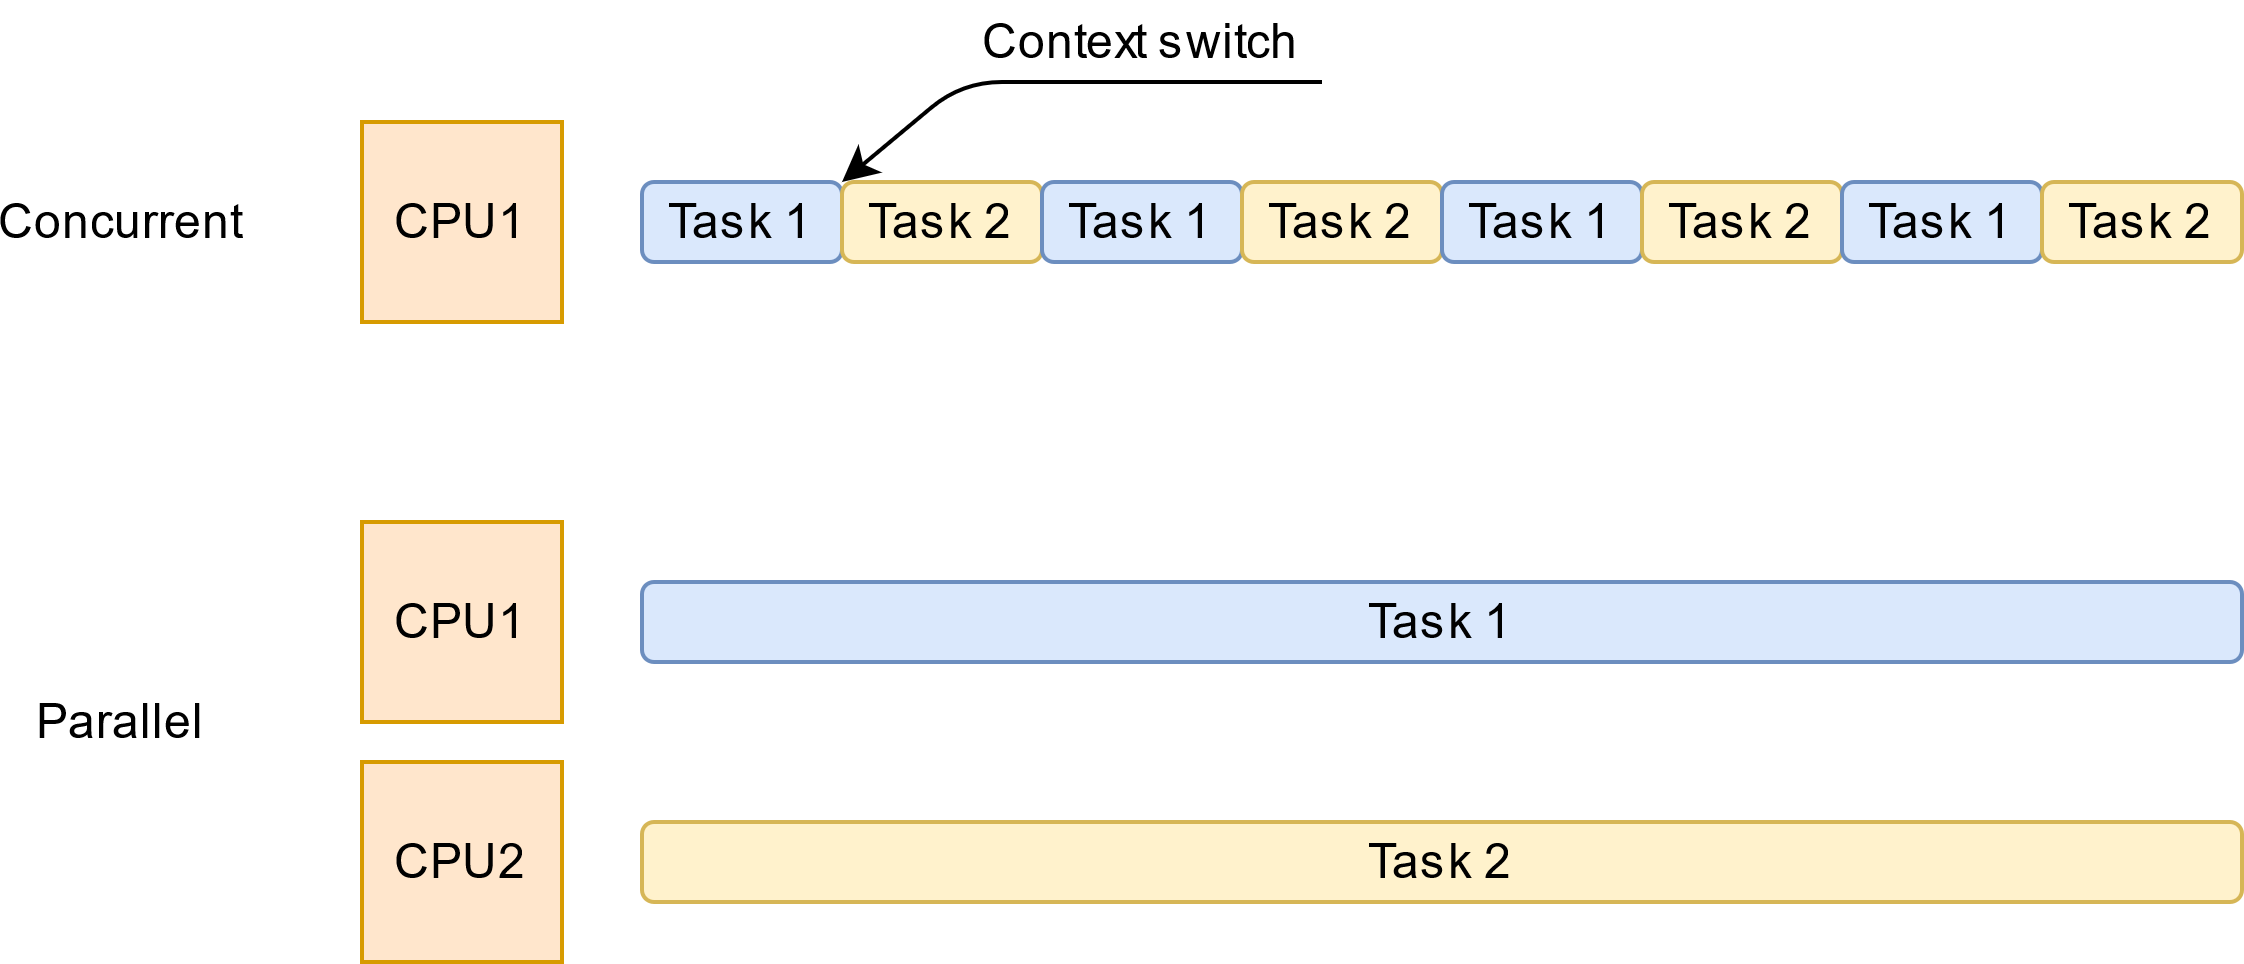
\includegraphics{figures02/convspar.png}
	\caption{Difference between concurrent and parallel models, both may look identical to the user}
	\label{fig:convspar}
\end{figure}

Concurrency is often confused with parallelism \cite{waza}, but concurrent programs only \emph{may} be executed in parallel 
by assigning each process to a separate processor or processor core, or distributing a computation across a network \cite{mordechai}

\subsection{Parallel programming}
Parallelism is the idea of processing tasks simultaneously, literally at the same time on different cores, for perfomance gains puroposes.

Although all parallel programs are concurrent, we have seen that not
all concurrency is parallel. That�s because parallelism depends on the actual runtime
environment, and it requires hardware support (multiple cores). Parallelism is achievable
only in multicore devices (figure 1.4) and is the means to increasing performance
and throughput of a program.
Parallelism can be achieved when a single task is split into multiple independent
subtasks, which are then run using all the available cores. In figure 1.5, a multicore
machine (two coffee stations) allows parallelism for simultaneously executing different
tasks (two busy baristas) without interruption.
The concept of timing is fundamental for simultaneously executing operations in
parallel. In such a program, operations are concurrent if they can be executed in parallel,
and these operations are parallel if the executions overlap in time

\begin{figure}[ht!]
	\centering
		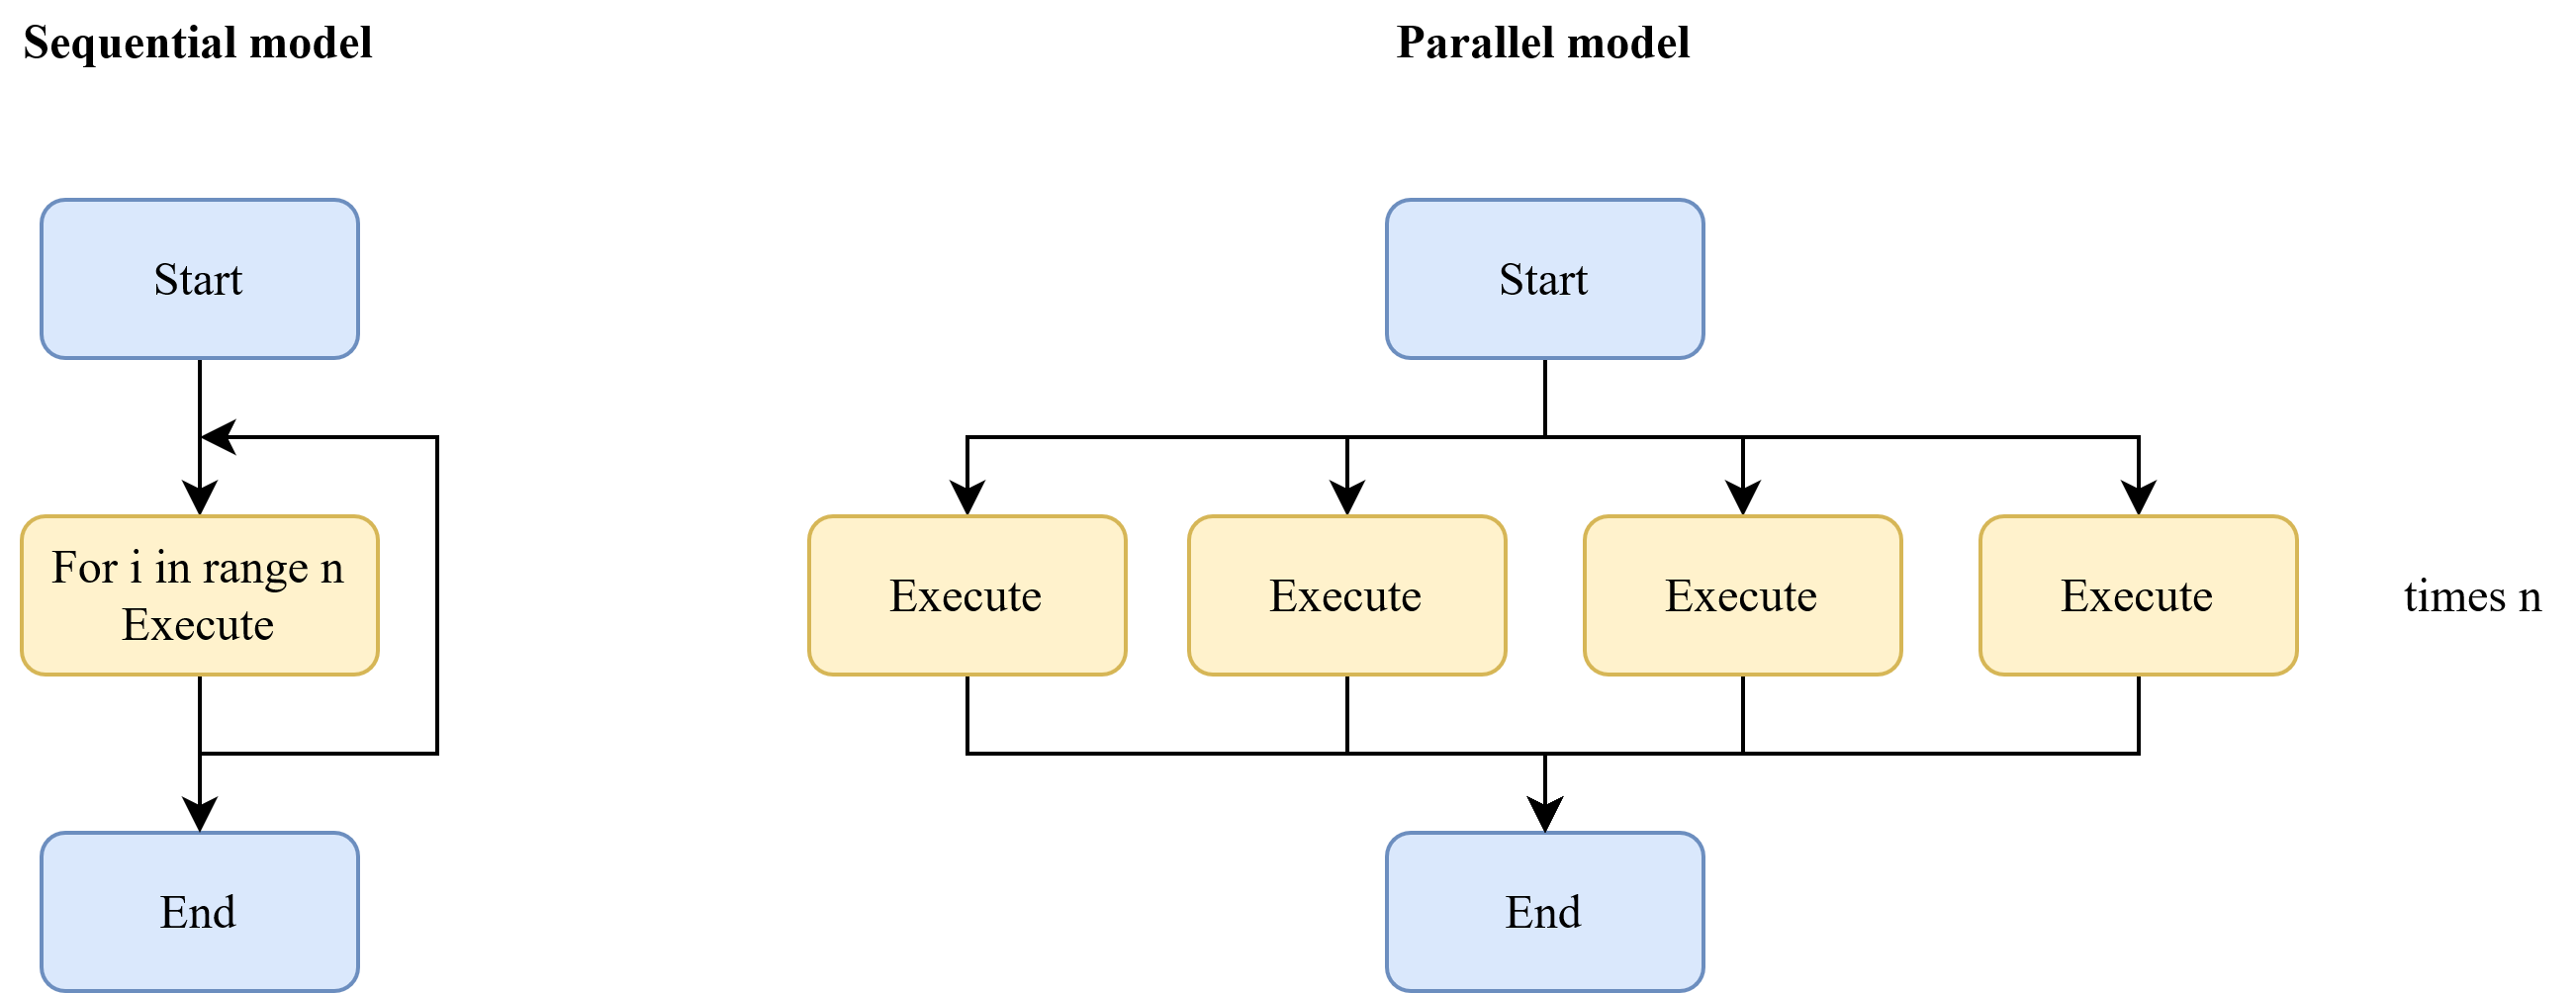
\includegraphics{figures02/seqvspar.png}
		\caption{Comparison of sequential and parallel models}
	\label{fig:seqvspar}
\end{figure}

\subsection{Multitasking}
Multitasking is the concept of performing multiple tasks over a period of time by executing
them concurrently. We�re familiar with this idea because we multitask all the
time in our daily lives. For example, while waiting for the barista to prepare our cappuccino,
we use our smartphone to check our emails or scan a news story. We�re doing
two things at one time: waiting and using a smartphone.
Computer multitasking was designed in the days when computers had a single CPU
to concurrently perform many tasks while sharing the same computing resources. Initially,
only one task could be executed at a time through time slicing of the CPU. (Time
slice refers to a sophisticated scheduling logic that coordinates execution between multiple
threads.) The amount of time the schedule allows a thread to run before scheduling
a different thread is called thread quantum. The CPU is time sliced so that each
thread gets to perform one operation before the execution context is switched to
another thread. Context switching is a procedure handled by the operating system to
Let�s start with terminology 11
multitask for optimized performance (figure 1.7). But in a single-core computer, it�s
possible that multitasking can slow down the performance of a program by introducing
extra overhead for context switching between threads.
Context switching on
a single-core machine
Figure 1.7 Each task has a different shade, indicating that the context switch in a single-core machine
gives the illusion that multiple tasks run in parallel, but only one task is processed at a time.
There are two kinds of multitasking operating systems:
? Cooperative multitasking systems, where the scheduler lets each task run until it finishes
or explicitly yields execution control back to the scheduler
? Preemptive multitasking systems (such as Microsoft Windows), where the scheduler
prioritizes the execution of tasks, and the underlying system, considering the priority
of the tasks, switches the execution sequence once the time allocation is
completed by yielding control to other tasks
Most operating systems designed in the last decade have provided preemptive multitasking.
Multitasking is useful for UI responsiveness to help avoid freezing the UI
during long operations.
\subsection{Multithreading}
Multithreading is an extension of the concept of multitasking, aiming to improve
the performance of a program by maximizing and optimizing computer resources.
Multithreading is a form of concurrency that uses multiple threads of execution.
Multithreading implies concurrency, but concurrency doesn�t necessarily imply multithreading.
Multithreading enables an application to explicitly subdivide specific tasks
into individual threads that run in parallel within the same process.
NOTE A process is an instance of a program running within a computer system.
Each process has one or more threads of execution, and no thread can exist
outside a process.
A thread is a unit of computation (an independent set of programming instructions
designed to achieve a particular result), which the operating system scheduler independently
executes and manages. Multithreading differs from multitasking: unlike
multitasking, with multithreading the threads share resources. But this �sharing
resources� design presents more programming challenges than multitasking does. We
discuss the problem of sharing variables between threads later in this chapter in section
1.4.1.
12 chapter 1 Functional concurrency foundations
The concepts of parallel and multithreading programming are closely related. But
in contrast to parallelism, multithreading is hardware-agnostic, which means that it can
be performed regardless of the number of cores. Parallel programming is a superset
of multithreading. You could use multithreading to parallelize a program by sharing
resources in the same process, for example, but you could also parallelize a program by
executing the computation in multiple processes or even
\section{Concurrency in .NET}
\chapter{Test Environment} 
\label{chap:3}
This chapter contains information about the test environment used in next chapters including description of benchmarking method and specification of hardware and software used in experiments. These parameters would be required if one set out to reproduce the collected data or to compare experiments conducted on different hardware or software.

\section{Benchmarking}
Tests performed in this paper will be constructed and executed using .NET benchmarking tool, \emph{BenchmarkDotNet}. It is an open source library which helps in transforming methods into benchmarks and producing reproducible experiments. The results are guaranteed to be reliable and precise by the usage of \emph{perfolizer} statistical engine. 

The tool is well equiped for the topic of this paper. It measures performance as mean estimated time, removes outlier data, calculates error ranges and standard deviation. Additionaly, \emph{MemoryDiagnoser} tracks GC generations and memory allocations which is important when testing parallel programs. Listing~\ref{lst:QSBenchClass} showcases one of the benchmarks which will be used during the experiments.
These benchmarks were developed with the use of \emph{Pro .NET benchmarking: the art of performance measurement} by Andrey Akinshin~\cite{Akinshin2019}.

\begin{lstlisting}[language={[sharp]c}, style=sharpcstyle, caption={Quicksort benchmark class}, label={lst:QSBenchClass}]
namespace Net47Benchmarking
{
  [SimpleJob(RuntimeMoniker.Net472)]
  [SimpleJob(RuntimeMoniker.NetCoreApp31)]
  [MemoryDiagnoser]
  [RPlotExporter]
  [CsvMeasurementsExporter]
  public class Net47QuickSortBenchmark
  {
    private readonly SequentialImperativeQuickSort _sequentialImperativeQuickSort = new SequentialImperativeQuickSort();
    private readonly ParallelImperativeQuickSort _parallelImperativeQuickSort = new ParallelImperativeQuickSort();
    private readonly OptimizedParallelImperativeQuickSort _optimizedParallelImperativeQuickSort =
      new OptimizedParallelImperativeQuickSort((int)Math.Log(Environment.ProcessorCount, 2) + 4);

    private readonly SequentialFunctionalQuickSort _sequentialFunctionalQuickSort = new SequentialFunctionalQuickSort();
    private readonly ParallelFunctionalQuickSort _parallelFunctionalQuickSort = new ParallelFunctionalQuickSort();
    private readonly OptimizedParallelFunctionalQuickSort _optimizedParallelFunctionalQuickSort =
      new OptimizedParallelFunctionalQuickSort((int)Math.Log(Environment.ProcessorCount, 2) + 4);

    // ReSharper disable once MemberCanBePrivate.Global
    public int[] Data;

    // ReSharper disable once MemberCanBePrivate.Global
    [Params(10000, 100000, 1000000, 10000000)] public int N;

    [GlobalSetup]
    public void Setup()
    {
      var random = new Random(42);

      Data = Enumerable
        .Range(0, N)
        .Select(_ => random.Next())
        .ToArray();
    }


    [Benchmark]
    public ImmutableList<int> SequentialFunctionalQuickSort()
       => _sequentialFunctionalQuickSort.Sort(Data).Result;

    [Benchmark]
    public ImmutableList<int> ParallelFunctionalQuickSort()
      => _parallelFunctionalQuickSort.Sort(Data).Result;

    [Benchmark]
    public ImmutableList<int> OptimizedParallelFunctionalQuickSort()
      => _optimizedParallelFunctionalQuickSort.Sort(Data).Result;

    [Benchmark]
    public ImmutableList<int> SequentialImperativeQuickSort()
      => _sequentialImperativeQuickSort.Sort(Data).Result;

    [Benchmark]
    public ImmutableList<int> ParallelImperativeQuickSort()
      => _parallelImperativeQuickSort.Sort(Data).Result;

    [Benchmark]
    public ImmutableList<int> OptimizedParallelImperativeQuickSort()
      => _optimizedParallelImperativeQuickSort.Sort(Data).Result;
  }
}
\end{lstlisting}


\clearpage
\section{Hardware and software} 
Each machine is different in it's own way, it is imperative to use the same hardware for all experiments to accurately benchmark tested software. Thus one cannot expect to receive the same results when conducting testing as presented later on this paper but in different settings. Specification of the machine used for development and benchmarking is presented in tab.~\ref{tab:HardSpec}. It's a middle-range (for 2021) machine for personal use.
\begin{table}[!ht]
    \centering
    \caption{Machine specification}
		\label{tab:HardSpec}
    \begin{tabular}{ll}
			\toprule
			CPU  & AMD Ryzen 5 3600 3.95 GHz 6 Cores 12 Logical Processors \\
			RAM  & Patriot 16GB 3000MHz CL16 \\ 
			MB   & Asus Prime X470 - Pro \\ 
			Disk & Samsung SSD 970 EVO Plus \\
			GPU  & AMD Radeon RX 5700 XT \\ 
			OS   & Windows 10 x64 Pro Build 19042 \\ 
			BIOS & American Megatrends 5406 \\ 
			\bottomrule
    \end{tabular}
\end{table}

AMD Ryzen 5 3600 is built using Zen2 architecture,  the successor of AMD's Zen and Zen+ microarchitectures. From the most notable features it enables 2 threads per physical core (SMT) and optimized processor caches: L1 cache with 32 kB  per core and 8-way associative input and output, L2 with 512 kB per core and L3 cache with 16MB per core. Fig.~\ref{fig:Zen} showcases microarchitecutre overview of Zen2 processors~\cite{Zen}.

\begin{figure}[!ht]
	\centering
		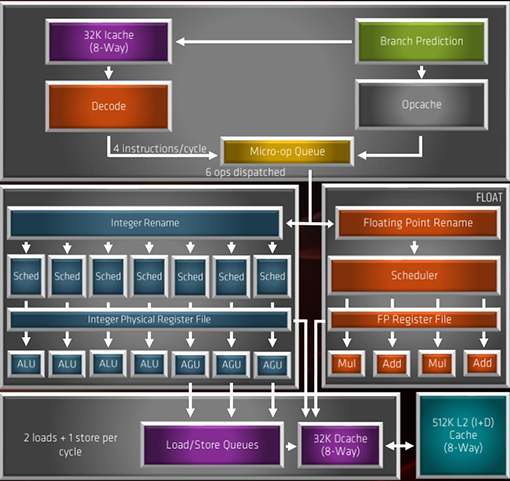
\includegraphics[width = 0.7\textwidth]{figures03/Zen.PNG}
	\caption{Zen2 microarchitecture}
	\label{fig:Zen}
\end{figure}

The aforementioned caches function as memory banks between main memory and the CPU. They store operation instructions and frequently used memory locations. The caches are usualy divided into three levels which are checked for hits in a top down manner:
\begin{itemize}
	\item \textbf{L1 cache} is the smallest, but the fastest cache. In case of Zen2 architecture it actually consists of two equal size caches, one for program data, second one for instructions. 
	\item \textbf{L2 cache} is next in line, it serves the same function as L1 but it is slightly bigger and slightly  slower.
	\item \textbf{L3 cache} is significantly bigger but accesing it will have  greater impact on performance. In Zen2 architecture this cache is shared between cores in one chiplet.  
\end{itemize}

Size and latency of the caches is presented on fig.~\ref{fig:Cache}.

\begin{figure}[!ht]
	\centering
		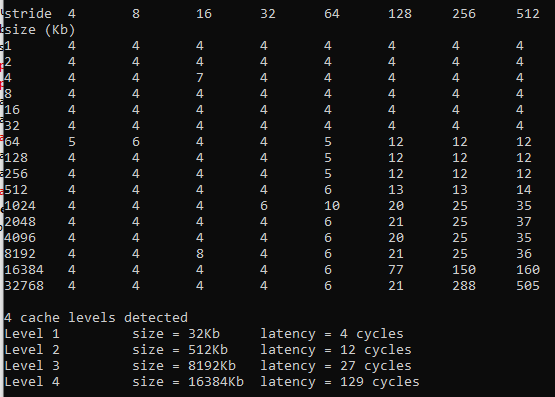
\includegraphics[width = 0.7\textwidth]{figures03/Cache.PNG}
	\caption{Ryzen 5 3600 cache sizes and latency}
	\label{fig:Cache}
\end{figure}

This chapter described how benchmarks will be conducted and specified hardware and software used in testing. Chapter that follows will introduce algorithms and software used in testing and their multiple implementations using parallel techniques. 

\chapter{Algorithms and software}
\section{Quicksort}

Quicksort pseudocode (shown in Lst. \ref{lst:PseudoQuickSort}) is based on description from \emph{Introduction to Algorithms} \cite{Cormen2009}.

\begin{lstlisting}[basicstyle=\ttfamily, caption={Sequential Quicksort pseudocode}, label={lst:PseudoQuickSort}]

QUICKSORT(A, p, r)
	if p < r
	q = PARTITION(A, p, r)
	QUICKSORT(A, p, q - 1)
  QUICKSORT(A, q + 1, r)
	
PARTITION(A, p, r)
	x = A[r]
	i = p - 1
  for j = p to r - 1
		if A[j] <= x
			i = i + 1
			exchange A[i] with A[j]
	exchange A[i + 1] with A[r]
	return i + 1
\end{lstlisting}

%\begin{lstlisting}[language={[Sharp]C}, caption={C\# exaple}, label={Script}]
%\end{lstlisting}

\clearpage
\chapter{Experiments}

\clearpage
\section{Mandelbrot}
Mandelbrot algorithm experiments were conducted using parameters presented in Tab. \ref{tab: MandelbrotParameters}. They describe amount of pixels generated and bitmap dimensions.
Sequential version of the algorithm had a MET  $\approx 5.6s$ . Parallel counterpart clocked at MET  $\approx 2.1s$, for a $\approx 62\%$ reduction. Parallel version with two \emph{Parallel.For} loops had a MET $\approx 2.7s$ which is $\approx 21\%$ slower than the less parallelized version using only one parallel loop. The best performing version using value type complex number had MET $\approx 1.9s$, for a $\approx 66\%$  reduction compared to sequential version and $\approx 11\%$  reduction to the parallel version. Additionaly, the value type version had 0 GC clean ups and virtually no (compared to others) memory consumption (Fig. \ref{fig: MandelbrotPerformance}, Tab. \ref{tab: MandelbrotBenchmarking}).

\begin{table}[!ht]
    \centering
    \caption{Mandelbrot benchmarking experiment parameters}
		\label{tab: MandelbrotParameters}
    \begin{tabular}{p{3cm}p{3cm}}
			\toprule
			\bfseries Name 	&
			\bfseries Value \\
			\midrule
			Width & 2.5 \\
			Height & 2.5 \\
			Column amount & 4000 \\ 
			Row amount  & 4000 \\	
			\bottomrule
    \end{tabular}
\end{table}

\begin{figure}[htb]
\centering
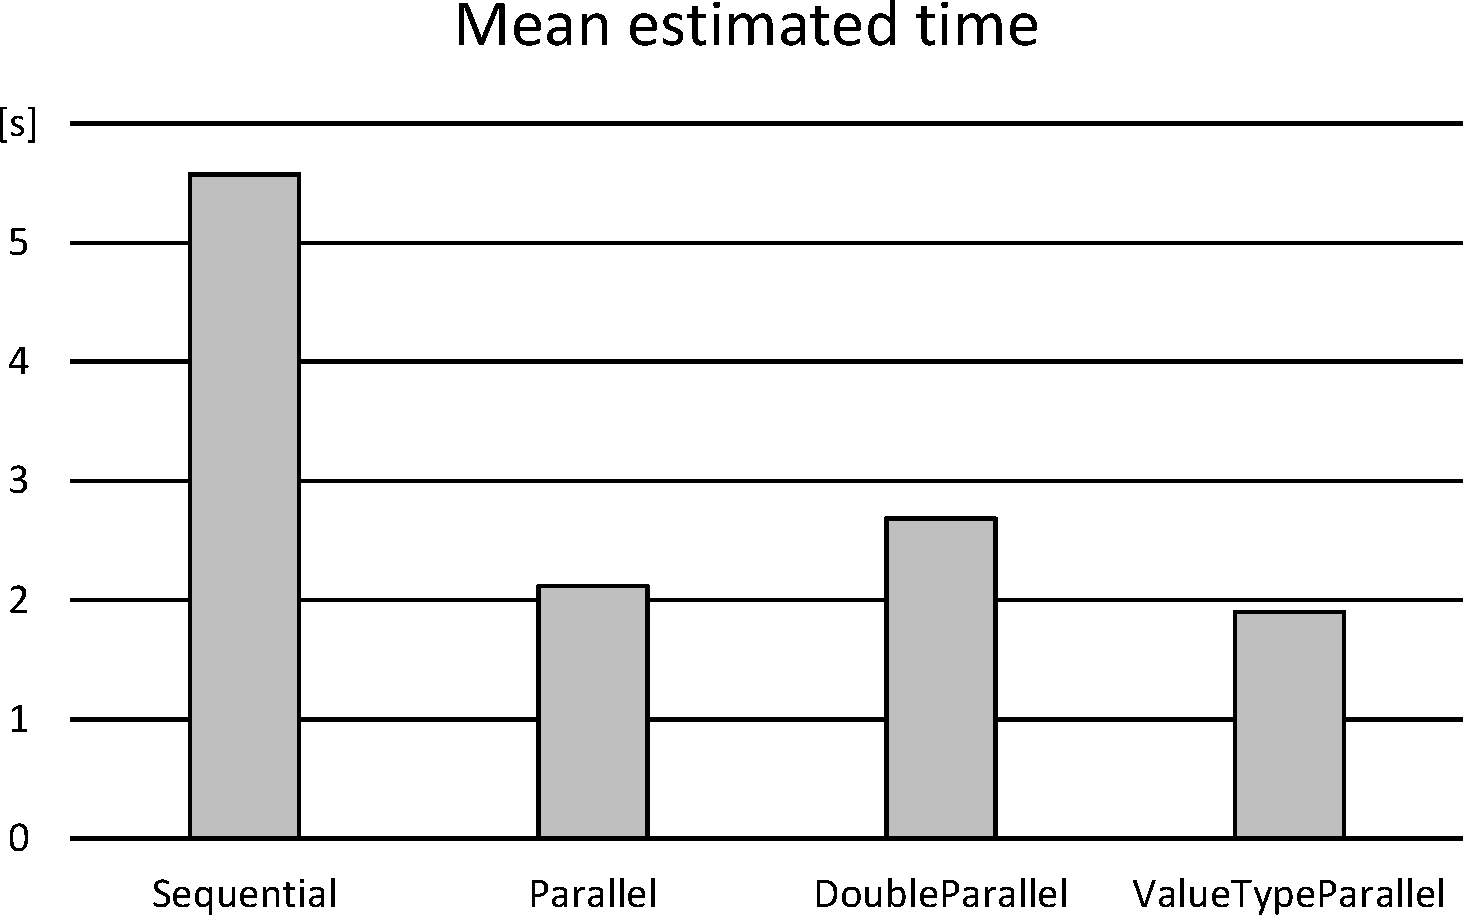
\includegraphics[width=.8\linewidth]{figures04/Fig41.pdf}
%%\begin{tikzpicture}
%%\begin{axis}[ symbolic x coords={
			%%Sequential, 
			%%Parallel, 
			%%DoubleParallel, 
			%%ValueTypeParallel, 
			%%DUMMY},
    %%xtick=data, 
		%%ylabel=Seconds,
    %%ybar interval=.7,
    %%enlargelimits=0.05]
    %%\addplot  coordinates {
      %%(Sequential, 5.576)
      %%(Parallel, 2.120)
      %%(DoubleParallel, 2.684)
      %%(ValueTypeParallel,1.903)
      %%(DUMMY, 0)
    %%};
     %%\legend{Mean estimated time}
%%\end{axis}
%%\end{tikzpicture}
\caption{Mandelbrot algorithm performance}
\label{fig: MandelbrotPerformance}
\end{figure}


\begin{table}[ht]%\small
    \centering
    \caption{Mandelbrot benchmarking results}
		\label{tab: MandelbrotBenchmarking}
    \begin{tabularx}{\linewidth}{Xrrrrrrr} \toprule
			\bfseries Version 	&
			\bfseries Mean    	&
			\bfseries Error	    &
			\bfseries StdDev	  &
			\bfseries Gen 0	    &
			\bfseries Gen 1	    &
			\bfseries Gen 2	    &
			\bfseries Allocated \\ \midrule
			Sequential & 5.576 s & 0.0564 s & 0.0528 s & 2483000 & 1000 & 1000 & 19851 MB \\ 
			Parallel & 2.120 s & 0.0458 s & 0.1350 s & 2485000 & 6000 & 1000 & 19843 MB \\ 
			DoubleParallel & 2.684 s & 0.0553 s & 0.1632 s & 2487000 & 39000 & 2000 & 19852 MB \\ 
			ValueTypeParallel & 1.903 s & 0.0137 s & 0.0128 s & 0 & 0 & 0 & 46 MB \\ 
			\bottomrule
	\end{tabularx}
\end{table}

\clearpage
\section{K-means clustering}
K-means clustering algorithm experiments were conducted using \emph{White wine quality} dataset \cite{WhiteWine}. Sequential version of the algorithm had MET $\approx 2.45s$ while the parallel one had MET $\approx 0.5s$, for a $\approx 80\%$ reduction at the cost of $\approx 18\%$ increase of memory consumption. Using partitioner further dropped down the MET to $\approx 0.43s$ which is a $\approx 82\%$ reduction from the sequential version and $\approx 15\%$ from the parallel one with equal memory consumption increase (Fig. \ref{fig: KMeansPerformance}, Fig. \ref{fig: KMeansMemory}, Tab. \ref{tab: KMeansBenchmarking}).

\begin{figure}[!ht]
\centering
\begin{tikzpicture}
\begin{axis}[ symbolic x coords={
			Sequential, 
			Parallel, 
			PartitionerParallel, 
			DUMMY},
    xtick=data, 
		ylabel=Miliseconds,
    ybar interval=.7,
    enlargelimits=0.05]
    \addplot  coordinates {
      (Sequential, 2453.7)
      (Parallel, 509.6)
      (PartitionerParallel, 434.5)
      (DUMMY, 0)
    };
     \legend{Mean estimated time}
\end{axis}
\end{tikzpicture}
\caption{K-means clustering  performance}
\label{fig: KMeansPerformance}
\end{figure}

\begin{figure}[!ht]
\centering
\begin{tikzpicture}
\begin{axis}[ symbolic x coords={
			Sequential, 
			Parallel, 
			PartitionerParallel, 
			DUMMY},
    xtick=data, 
		ylabel=Megabytes,
    ybar interval=.7,
    enlargelimits=0.05]
    \addplot[fill=gold]  coordinates {
      (Sequential, 151)
      (Parallel, 183)
      (PartitionerParallel, 184)
      (DUMMY, 0)
    };
     \legend{Memory consumption}
\end{axis}
\end{tikzpicture}
\caption{K-means clustering memory consumption}
\label{fig: KMeansMemory}
\end{figure}

\begin{table}[ht]%\small
    \centering
    \caption{K-means clustering benchmarking results}
		\label{tab: KMeansBenchmarking}
    \begin{tabularx}{\linewidth}{Xrrrrrrr} \toprule
			\bfseries Version 	&
			\bfseries Mean    	&
			\bfseries Error	    &
			\bfseries StdDev	  &
			\bfseries Gen 0	    &
			\bfseries Gen 1	    &
			\bfseries Gen 2	    &
			\bfseries Allocated \\ 
			\midrule 
Sequential & 2,453.7 ms	& 25.01ms	& 20.89ms	& 18000 & 	2000 & 	0 & 151 MB \\
Parallel & 509.6 ms	& 8.28 ms	& 8.50 ms	& 23000 & 	9000 & 	0 & 183 MB \\ 
PartitionerParallel & 434.5 ms	& 2.69 ms	& 2.52 ms	& 23000 & 	8000 & 	0 & 184 MB \\
			\bottomrule
    \end{tabularx}
\end{table}
\chapter{Discussion}
After carefully designing the experiments in chapter~\ref{chap:3} and \ref{chap:4} and conducting them in chapter\ref{chap:5} this part will discuss the outcomes of the benchmarks. 
After interpreting and analyzing the results, a set of guidelines for future .NET parallel ventures will be presented. \\
 
At the stage of development of algorithms and software it quickly became clear that benchmarking is crucial when programming for performance. 
Sometimes a small tweak in unimportant subroutine would completely change the speed of execution, thus many iterations of the code were discarded even before the experiments proper. 
Some of these haphazard implementations were included in QuickSort part (section~\ref{sec: QuickSort}). Async-await state machine is an useful construct, but it was build for fluidity of applications, not for performance. Without benchmarking such code might have slipped into production environment for a potential disaster. \emph{BenchmarkDotNet} enables programmers
to scale-back the tests so they can be used during development or even use them as part of their unit test suite.

Platform version is very significant when it comes to performance. .NET, thanks to being open source, is often updated with small fixes and improvements which aren't always included in the major release notes. Such updates may have big impact on the application, especially if it uses high-level constructs like LINQ. This was confirmed by tests conducted in QuickSort part (section~\ref{sec: QuickSort}). Switching from .NET Framework 4.7 to .NET Core 3.1 brought major improvements across all versions of the algorithm. Further test were conducted only with .NET Core 3.1 since the first example was enough to drive the point.

Another point that came out of QuickSort part (section~\ref{sec: QuickSortImp}) is that specific implementation matters. Imperative version of the algorithm highly overperformed the functional one and didn't benefit as much from parallelisation. The cost in this case came from other factors: length of the implementation, understandability and reliability. Imperative version took many iterations to get just right, even with something relatively simple as the QuickSort algorithm. The end result is convoluted, hard to read and understand piece of software. On the other hand, version using LINQ was simple to write and end result is comprehensive and concise. Any further maintenance over this version would be significantly easier. One has to consider cost-benefit of programming for performance when choosing the specific implementation. 

When using parallelism it is important to gauge the amount of tasks spawned by the software. Otherwise, resource heavy context switches will overhelm any potential speed benefits of parallel programming. This was demonstrated in QuickSort algorithm (section~\ref{sec: QuickSort}) and Mandelbrot set drawing (section~\ref{sec: Mandelbrot}). In the former, lack of depth control together with async-await rendered the implementation completely inefficient. In the latter, using two nested \emph{Parallel.For} loops performed worse than using only one. We can hypothesize that further parallelisation would decrease the performance even more. 

Data parallelism Fork/Join and MapReduce patterns proved to be useful and powerful. The former was used in the implementation of K-Means algorithm (section~\ref{sec: KMeansImp}) and the latter in software ranking NuGet packages (section~\ref{sec: NuGetImp}). Both of these patterns can be implemented in a generic way, allowing programmers to drop them in when they see fit. Parallelisation was again streamlined thanks to the use of LINQ, turning the queries into parallel ones required few PLINQ lines. This makes the code clear and easy to understand, on contrary to often convoluted parallel implementations. 

Load balancing with a data partitioner is a strategy worth considering when implementing parallel queries. This addition was especially performant with larger datasets in NuGet package ranking software (section~\ref{sec: NuGet}), not so much with smaller datasets like in the case of Madelbrot algorithm (section~\ref{sec: Mandelbrot}). 

Almost all parallel implementations came with a cost of memory consumption oscillating around 15\%. Considering that memory is abundant in modern computing machines, this shouldn't be an important factor unless working on a device which has for some reasons significant memory constraints. Special case can be made for algorithm which allocate a lot of memory by object creation, as in the case of Mandelbrot algorithm (section~\ref{sec: MandelbrotImp}) which creates millions of objects inside its functions. When Garbage Collector cleanups become the bottleneck and stop the program from executing, it might be worth to consider using value types structures instead (section~\ref{sec: Mandelbrot}).\\

To summarize this analysis: 
\begin{itemize}
	\item Benchmarking is crucial at all stages of development.
	\item \emph{BenchmarkDotNet} is recommended as the go to library for .NET benchmarking.
	\item Modern platforms are optimized for performance, working on newest versions should be a~priority.
	\item Parallel programs should be written with understandability, reliability and maintainability in mind. Functional paradigm offers great tools which enable this goal.
	\item Depth of parallelisation should always be controlled for, exact numbers should be data driven.
	\item Fork/Join and MapReduce patterns are recommended in data parallelism problems. 
	\item Data load balancing with partitioners is recommended for large datasets.
	\item Do not preemptively optimize for memory consumption unless it is required by specific scenario.
	\item If scenario includes creating many objects inside local function scope, consider using value type instead of reference type.

\end{itemize}


%\bibliographystyle{plalpha}
\bibliographystyle{abbrv}
% \bibliographystyle{plain}

%Warning: References should be collected in a separate file. You can use the programm JabRef for editing. 
%         But please remember, that not all JabRef types of entries are supported by BibTeX.
%         File name below is given without extenion 
%         (here BibTeX will look for "bibiography.bib" in the main directory)
\setlength{\bibitemsep}{2pt} % introduced to make smaller seps between bibliographic items
\bibliography{bibliography}
\appendix
\chapter{Layout of attached CD/DVD}

The attached CD contains following files:
\begin{itemize}
	\item \texttt{W04\_235405\_2021\_praca magisterska.pdf} - PDF file containing the master thesis with abstract and appendixes.
	\item \texttt{Source Code} - folder containing source code used in this thesis:
	\begin{itemize}
		\item \texttt{MasterThesis.sln} - solution file, this can be opened via Visual Studio 19.
		\item \texttt{Algorithms} - folder containing all implementations of algorithms and software.
		\item \texttt{NugetDownloader} - folder containing NuGet package downloader.
		\item \texttt{Benchmarking} - folder containing .NET Core 3.1 benchmark classes.
		\item \texttt{Net47Benchmarking} - folder containing .NET Framework 4.7 benchmark classes.
	\end{itemize}
	\item \texttt{Executables} - folder containing shortcuts to benchmarking executables.
\end{itemize}

To run the benchmarks it is required to have installed:
\begin{itemize}
	\item .NET Framework 4.7
	\item .NET Core 3.1
\end{itemize}

Afterwards, the benchmarks can be run via \texttt{Benchmarking.exe} and \texttt{Net47Benchmarking.exe}.
Alternatively, one can open \texttt{MasterThesis.sln} in Visual Studio 19 and recompile the source code,
the benchmarks are set as startup projects automatically executed after each build.

\chapter{Layout of attached CD/DVD}
% Please describe here the content of attached CD (normally there should be pdf with the thesis text and folders, including sources of software project if any).



%%Uncomment the lines below, if you want to use index
%%\chapterstyle{noNumbered}
%%\phantomsection 
%%\addcontentsline{toc}{chapter}{Index}
%%\printindex

\end{document}
